%%
% TUM Corporate Design LaTeX Templates
% Based on the templates from https://www.tum.de/cd
%
% Feel free to join development on
% https://gitlab.lrz.de/tum-templates/templates
% and/or to create an issue in case of trouble.
%
% tum-presentation class for scientific talks, thesis presentations, ...
%
%%

%\documentclass[4to3]{tum-presentation}
%\documentclass[navsym]{tum-presentation}
%\documentclass[nothreeliner]{tum-presentation}
%\documentclass[handout,4on1]{tum-presentation}
%\documentclass[handout,2on1]{tum-presentation}
%\documentclass[handout]{tum-presentation}
\documentclass{tum-presentation}

\addbibresource{literature.bib}

\title[Shortened Title]{Clustering-Based Sentiment Analysis for Media Agenda Setting}
\subtitle{Opinion Lab Group 2.3}
\author{Wing Sheung Leung, Qiaoxi Liu}
%\institute[]{\inst{1} Department of Electrical and Computer Engineering,
%  Technical University of Munich (TUM)\\
%  \inst{2} Department of Informatics, Technical University of Munich (TUM)}
%\date{International Conference on Mostly Scientific Topics}

\footline{\insertshortauthor~| \inserttitle}

\begin{document}

\begin{frame}[noframenumbering]
  \titlepage
\end{frame}

\begin{frame}
  \frametitle{Outline}
  \large
  \begin{itemize}
  \item Aims
  \item Dataset
  \item Expected outputs
  \item Todo
    \begin{itemize}
        \item Stage 1
        \begin{itemize}\normalsize
            \item Generate word / token / sentence embeddings with our corpus
            \item Build a k-mean clustering model for identifying sub-topics in organic dataset
            \item Select a sentiment pre-trained model
        \end{itemize}
        \item Stage 2
        \begin{itemize}\normalsize
            \item Visualize distribution of samples among clusters and corresponding sentiment frequency
        \end{itemize}
        \item Stage 3
        \begin{itemize}\normalsize
            \item Investigate Media Agenda Setting
        \end{itemize}
    \end{itemize}
  \item Milestones
  \end{itemize}

\end{frame}

\begin{frame}
  \frametitle{Aims}
  \large
  \begin{description}
    \item \textbf{Measure the influence of two online newspapers onto the social media according to Agenda setting theory}
    \vspace{1cm}
    \item \underline{Agenda setting theory}:
    \item Suggest the news item which is covered more frequently and prominently indicates that the audience will regard the issue as more important.
  \end{description}
\end{frame}

\begin{frame}
  \frametitle{Dataset}
  \large
  \begin{description}
    \item Articles and respective comments on the domain of organic food with search terms \emph{organic food} and \emph{organic farming}
    \begin{itemize}
      \item Articles from two online newspapers, \emph{New York Times} (English) and \emph{Der Spiegel} (German)
      \item 
      \underline{Direct response (bilingual)}: comments right under those articles
      \item 
      \underline{Indirect response}: posts in unrelated discussion forums, \emph{Quora}
    \end{itemize}
  \end{description}
  \small
  \begin{table}[t]
    \begin{tabular}{lcccc}
    \hline
    & Start & End & No. of articles\\
    \hline
    \emph{New York Times}\\ 
    \hline
    With comments & 2006 & 2017 & 99\\
    Without comments & 1970 & 2017 & 228\\
    \hline
    \emph{Der Spiegel}\\
    \hline
    With comments & 2007 & 2017 & 61\\
    Without comments & 2007 & 2017 & 91\\
    \hline
    \emph{Quora}\\
    \hline
    With comments & 2009 & 2017 & 1304\\
    Without comments & 2010 & 2017 & 193\\
    \hline
    \end{tabular}
    \caption{Statistics for data crawled from New York Times, Der Spiegel and Quora with 'relevant' labelled as 1.0}
    \label{ex:table}
  \end{table}
\end{frame}

\begin{frame}
  \frametitle{Expected outputs (Processes)}

  \begin{figure}[t]
    \centering
        \begin{tabular}{ccc}
            \begin{minipage}[t]{2.8in}
            
\includegraphics[width=3in]{images/expect-output-1.png}
            \caption{Stage 1: Cluster, tuple(aspect,sentiment) }
            \end{minipage}
          $\to$
            \begin{minipage}[t]{2.5in}
            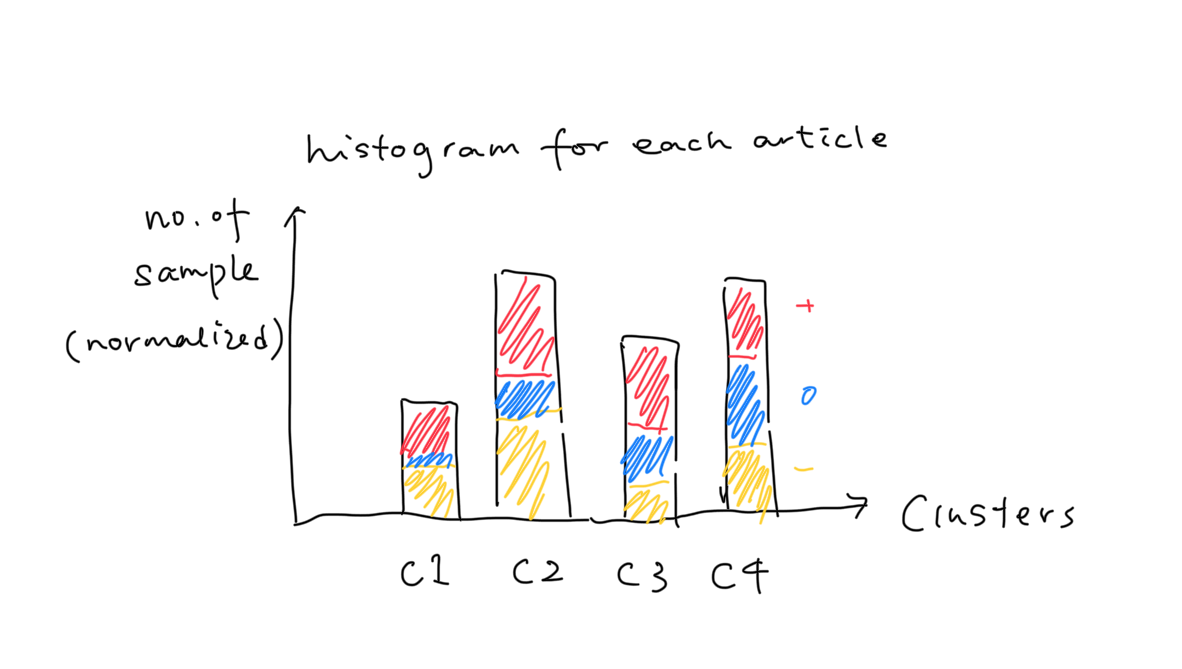
\includegraphics[width=3in]{images/expect-output-3.png}
            \caption{Stage 2: Distribution of clusters per articles}
            \end{minipage}
        $\to$
        \begin{minipage}[t]{2.8in}
              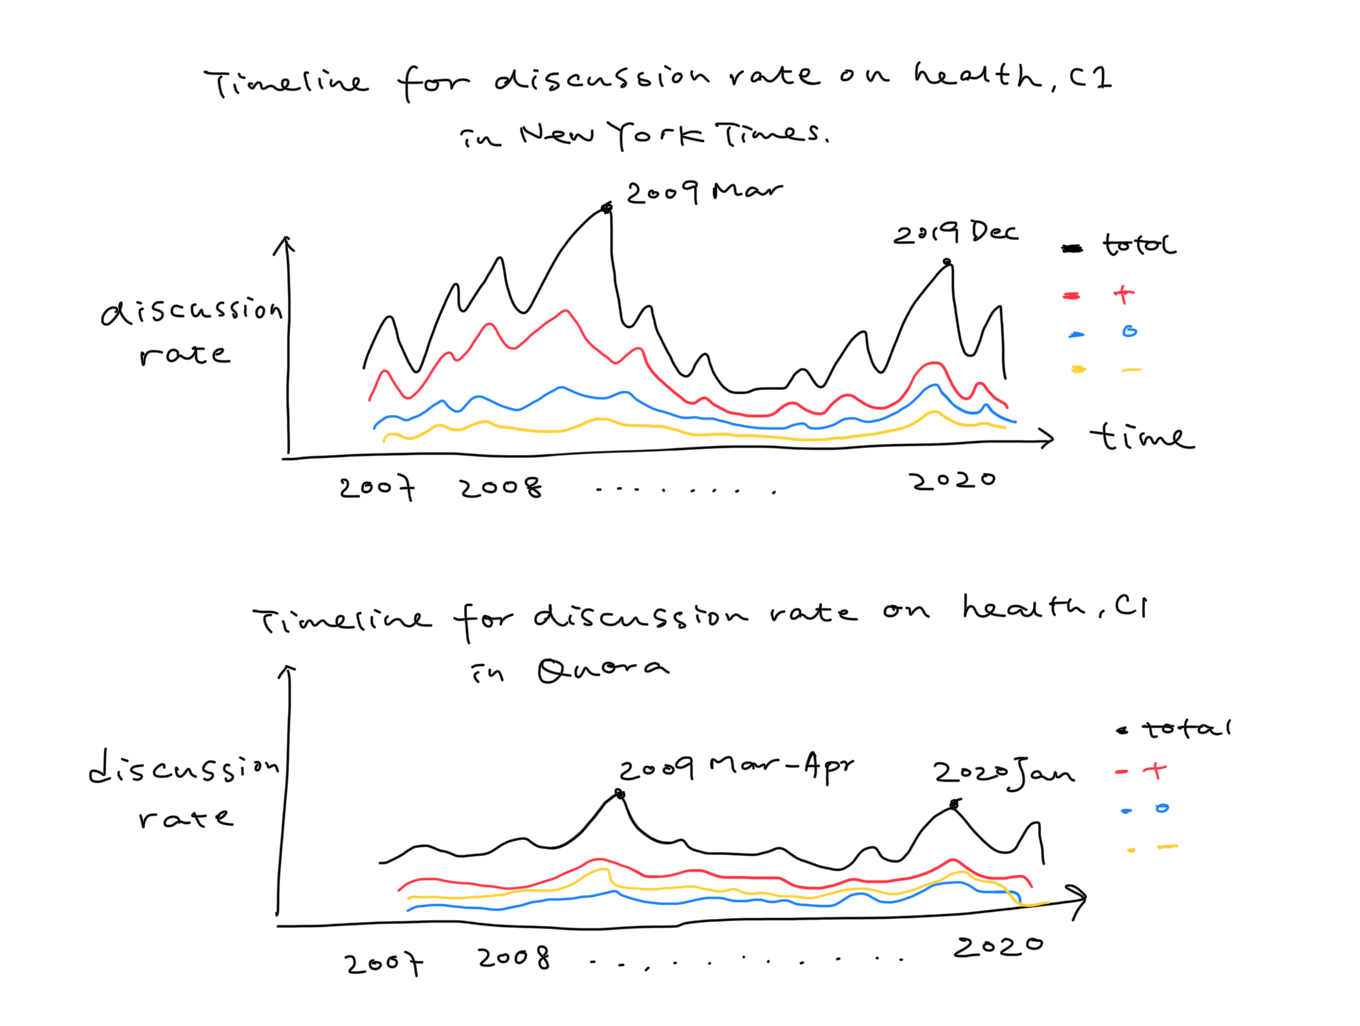
\includegraphics[width=3in]{images/expect-output-4.png}
              \caption{Stage 3: Timeline analysis, influence on social media}
              \end{minipage}
        \end{tabular}
    \end{figure}
   

\end{frame}

\begin{frame}[fragile]
  \frametitle{Todo Stage 1.1}
  \framesubtitle{Generate embeddings }

  \begin{description}
    \item \textbf{text}  $\to$ \textit{lines split}  $\to$ list of sentences $\to$ \textit{sentence embedding}  $\to$ \textbf{vectors}
   
    \pause 
    \vspace{0.2cm}
    \item \underline{Example:} $sentence=$"You are what you eat." 
    \vspace{0.2cm}
    \pause 
    \item Possible embedding models (on TensorFlow Hub) to apply:
    \begin{itemize}
      \item  Universal sentence encoder \footcite{chidambaram2018learning}
      \item  Bert \footcite{bertontfhub}
    \end{itemize}
    \pause 
  \begin{lstlisting}
embed = hub.Module("https://tfhub.dev/google/universal-sentence-encoder-xling/en-de/1")
with tf.Session() as session:
  session.run()
  print(session.run(embed(sentence)))
    \end{lstlisting}
    \item $ \to [0.02, 0.01, ..., -0.12]$
  \end{description}
\end{frame}

\begin{frame}[fragile]
  \frametitle{Todo Stage 1.2}
 \framesubtitle{Build a k-mean clustering model for identifying sub-topics}
 \begin{description}
  \item Now, let's start working with \textbf{vectors}! 

  \item $\to$ k-means cluster, optimize k with human observation \alert{(samples: sentences)}
  \pause 
  \begin{lstlisting}
  s_emb_matrix = [s0, s2, ..., s9] # s are embedding vectors of sentences
  nclusters= 3
  km = KMeans(nclusters)
  km.fit(s_emb_matrix)
  clusters = {} # key: label, values: index of sentence
  for i, label in enumerate(km.labels_):
    clusters[label].append(i) # append the index to the corresponding label
  \end{lstlisting}
  \pause 
    \item $\to$ get $clusters[0]:s_0,s_4,s_5$ with top-n words list $topWords[0]:w_0,w_1,...w_n$
    \pause 
    \item $\to$ under each cluster, check similarities of words  \alert{(samples: words)}
    \pause 
    \item $\to$ interpret/extract $clusters[0]$ to an aspect (like environment).
    \item  $\to$ sentences $s_0,s_4,s_5$ are assigned to environment.
  \end{description}

\end{frame}


\begin{frame}[fragile]
  \frametitle{Todo Stage 1.3}
  \framesubtitle{Select a sentiment pre-trained model }
  \begin{description}
    \item Since we get $s_0$ $\to$ "environment", we use pre-trained VADER classifier\footcite{hutto2014vader}
    \item for each sentence, output a \textbf{2-tuple}.
    \pause 
    \vspace{0.3cm}
    \item \underline{Example}
    \item $s_0=$"not only improves the fruit quality, but is a lot better on our environment as well."
    \pause 
    \vspace{0.2cm}
    \item $\to$ arr = [0.2,...,0.1] $\to$ \textit{kmean clustering}  $\to$  "Environment" (result from stage 1.2)
    \pause 
    \item $\to$ \textit{VADER classifier}
    \begin{lstlisting}
    analyzer = SentimentIntensityAnalyzer()
    print(analyzer.polarity_scores(arr))
  \end{lstlisting}
  \item $\to$ \{\textbf{'pos': 0.74}, 'neu': 0.26, 'neg': 0.0\}
  \pause 
  \item $\to$ \textbf{(Environment, pos)}
  \end{description}
\end{frame}

\begin{frame}
  \frametitle{Todo Stage 2}
  
 \framesubtitle{Visualize distribution on single article (and its comments) }
 \begin{description}
  \item Now, the sentence $s$ is converted into a tuple $t=(Aspect, +/-/o)$ . 
  \pause 
  \item $\to$ Take all samples $[t_0, t_1, t_2, ...]$ from one article
  \item $\to$ accumulate and normalize them
  \pause 
\end{description}
\begin{figure}[t]
  
 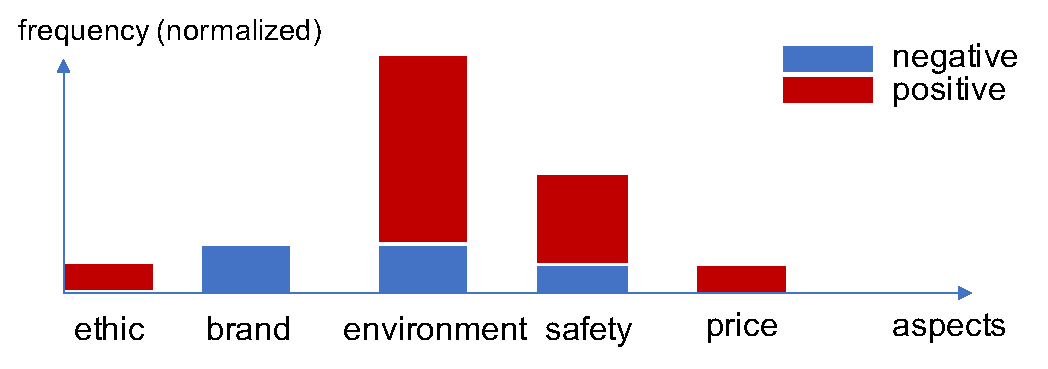
\includegraphics[width = 0.5\textwidth]{figures/distribution.pdf}
 \caption{Aspects distribution on one text}
 \end{figure}
\end{frame}

\begin{frame}
  \frametitle{Todo Stage 3}
 \framesubtitle{Investigate Media Agenda Setting}
 \begin{description}
  \large
  \item \textbf {Does $Y$ (news) has influence on $X$ (comments/Quora)? }
  \pause 
  \normalsize
  \item $\to$ discover/measure the relationship between X,Y
  \begin{itemize}
  \item Pearson correlations (time not considered)
  \item Local Similarity Analysis (LSA) statistic identifies the existence of local and lagged relationships
  \item Granger causality (Does $Y_t$ help to predict $X_{t+1}$ ?)
  \item Lagged Correlation (response after a lapse of time, how strong correlation)
  
  \end{itemize}
  \pause 
\begin{figure}[]
  \centering
  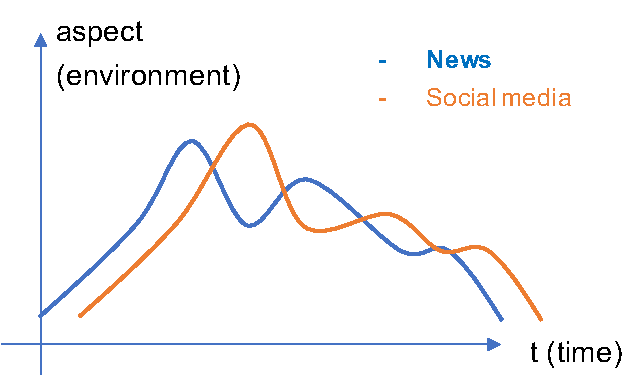
\includegraphics[width = 0.4\textwidth]{figures/timecor.pdf}
  %\caption{}
  \label{}
\end{figure}
 

\end{description}
\end{frame}

\begin{frame}
  \frametitle{Milestones}
  \vspace{2cm}
 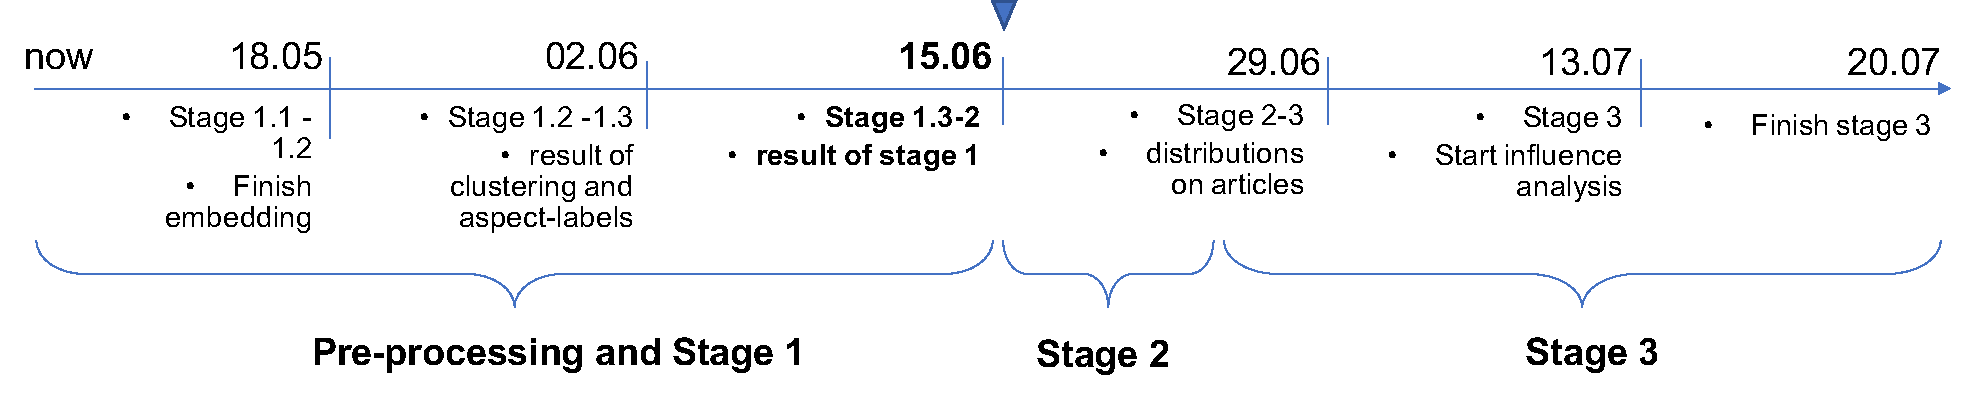
\includegraphics[width = \textwidth]{figures/timeline.pdf}
  
\end{frame}


\begin{frame}
  \frametitle{References}
 
  \printbibliography

\end{frame}

\end{document}
